\documentclass[twoside]{book}

% Packages required by doxygen
\usepackage{fixltx2e}
\usepackage{calc}
\usepackage{doxygen}
\usepackage[export]{adjustbox} % also loads graphicx
\usepackage{graphicx}
\usepackage[utf8]{inputenc}
\usepackage{makeidx}
\usepackage{multicol}
\usepackage{multirow}
\PassOptionsToPackage{warn}{textcomp}
\usepackage{textcomp}
\usepackage[nointegrals]{wasysym}
\usepackage[table]{xcolor}

% Font selection
\usepackage[T1]{fontenc}
\usepackage[scaled=.90]{helvet}
\usepackage{courier}
\usepackage{amssymb}
\usepackage{sectsty}
\renewcommand{\familydefault}{\sfdefault}
\allsectionsfont{%
  \fontseries{bc}\selectfont%
  \color{darkgray}%
}
\renewcommand{\DoxyLabelFont}{%
  \fontseries{bc}\selectfont%
  \color{darkgray}%
}
\newcommand{\+}{\discretionary{\mbox{\scriptsize$\hookleftarrow$}}{}{}}

% Page & text layout
\usepackage{geometry}
\geometry{%
  a4paper,%
  top=2.5cm,%
  bottom=2.5cm,%
  left=2.5cm,%
  right=2.5cm%
}
\tolerance=750
\hfuzz=15pt
\hbadness=750
\setlength{\emergencystretch}{15pt}
\setlength{\parindent}{0cm}
\setlength{\parskip}{3ex plus 2ex minus 2ex}
\makeatletter
\renewcommand{\paragraph}{%
  \@startsection{paragraph}{4}{0ex}{-1.0ex}{1.0ex}{%
    \normalfont\normalsize\bfseries\SS@parafont%
  }%
}
\renewcommand{\subparagraph}{%
  \@startsection{subparagraph}{5}{0ex}{-1.0ex}{1.0ex}{%
    \normalfont\normalsize\bfseries\SS@subparafont%
  }%
}
\makeatother

% Headers & footers
\usepackage{fancyhdr}
\pagestyle{fancyplain}
\fancyhead[LE]{\fancyplain{}{\bfseries\thepage}}
\fancyhead[CE]{\fancyplain{}{}}
\fancyhead[RE]{\fancyplain{}{\bfseries\leftmark}}
\fancyhead[LO]{\fancyplain{}{\bfseries\rightmark}}
\fancyhead[CO]{\fancyplain{}{}}
\fancyhead[RO]{\fancyplain{}{\bfseries\thepage}}
\fancyfoot[LE]{\fancyplain{}{}}
\fancyfoot[CE]{\fancyplain{}{}}
\fancyfoot[RE]{\fancyplain{}{\bfseries\scriptsize Generated by Doxygen }}
\fancyfoot[LO]{\fancyplain{}{\bfseries\scriptsize Generated by Doxygen }}
\fancyfoot[CO]{\fancyplain{}{}}
\fancyfoot[RO]{\fancyplain{}{}}
\renewcommand{\footrulewidth}{0.4pt}
\renewcommand{\chaptermark}[1]{%
  \markboth{#1}{}%
}
\renewcommand{\sectionmark}[1]{%
  \markright{\thesection\ #1}%
}

% Indices & bibliography
\usepackage{natbib}
\usepackage[titles]{tocloft}
\setcounter{tocdepth}{3}
\setcounter{secnumdepth}{5}
\makeindex

% Hyperlinks (required, but should be loaded last)
\usepackage{ifpdf}
\ifpdf
  \usepackage[pdftex,pagebackref=true]{hyperref}
\else
  \usepackage[ps2pdf,pagebackref=true]{hyperref}
\fi
\hypersetup{%
  colorlinks=true,%
  linkcolor=blue,%
  citecolor=blue,%
  unicode%
}

% Custom commands
\newcommand{\clearemptydoublepage}{%
  \newpage{\pagestyle{empty}\cleardoublepage}%
}

\usepackage{caption}
\captionsetup{labelsep=space,justification=centering,font={bf},singlelinecheck=off,skip=4pt,position=top}

%===== C O N T E N T S =====

\begin{document}

% Titlepage & ToC
\hypersetup{pageanchor=false,
             bookmarksnumbered=true,
             pdfencoding=unicode
            }
\pagenumbering{roman}
\begin{titlepage}
\vspace*{7cm}
\begin{center}%
{\Large E\+E\+CS 448 Project \\[1ex]\large 1 }\\
\vspace*{1cm}
{\large Generated by Doxygen 1.8.11}\\
\end{center}
\end{titlepage}
\clearemptydoublepage
\tableofcontents
\clearemptydoublepage
\pagenumbering{arabic}
\hypersetup{pageanchor=true}

%--- Begin generated contents ---
\chapter{Works Cited}
\label{Citations}
\hypertarget{Citations}{}
List of resources, code, and tutorials we used along the way

\begin{DoxyAuthor}{Author}
Grant Jurgensen, Stephen Longofono, Stephen Wiss
\end{DoxyAuthor}
\hypertarget{Citations_Citations}{}\section{Citations}\label{Citations_Citations}
\hypertarget{Citations_one}{}\subsection{Leap Year Algorithm}\label{Citations_one}
An algorithm to determine if it is a leap year, adapted from the logic shown in this wikipedia page\+: Accessed September, 2016, \href{https://en.wikipedia.org/wiki/Leap_year#Algorithm}{\tt https\+://en.\+wikipedia.\+org/wiki/\+Leap\+\_\+year\#\+Algorithm}\hypertarget{Citations_two}{}\subsection{Day of the Week Algorithm}\label{Citations_two}
An algorithm to determine the day of the week of the first day of the year, adapted from the algortihm on the \char`\"{}disparate variation\char`\"{} of Gauss\textquotesingle{}s algorithm, shown here\+: Accessed September, 2016, \href{https://en.wikipedia.org/wiki/Leap_year#Algorithm}{\tt https\+://en.\+wikipedia.\+org/wiki/\+Leap\+\_\+year\#\+Algorithm}\hypertarget{Citations_three}{}\subsection{Regular Expressions}\label{Citations_three}
Regular expressions were built for date parsing using a tutorial written by Jan Goyvaerts. Accessed September 2016, \href{https://www.regular-expressions.info/dates.html}{\tt https\+://www.\+regular-\/expressions.\+info/dates.\+html}\hypertarget{Citations_four}{}\subsection{Flask Extensions \& Best Practices}\label{Citations_four}
We consulted the official Flask documentation while writing our server, and adapted many of the examples to fit our needs. Since much of what we used was simply T\+HE way to implement any given feature, we did not cite them individually within the code.

Flask Documentation by Armin Ronacher, Accessed September 2016, \href{http://flask.pocoo.org/docs/0.11/}{\tt http\+://flask.\+pocoo.\+org/docs/0.\+11/}\hypertarget{Citations_five}{}\subsection{Flask Micro-\/\+Blog Tutorial}\label{Citations_five}
This extensive tutorial was used as a model for our authentication, and was also where we got the Bootstrap code for our client-\/side C\+SS.

The Flask Mega-\/\+Tutorial by Miguel Grinberg, Accessed September 2016, \href{http://blog.miguelgrinberg.com/post/the-flask-mega-tutorial-part-i-hello-world}{\tt http\+://blog.\+miguelgrinberg.\+com/post/the-\/flask-\/mega-\/tutorial-\/part-\/i-\/hello-\/world}\hypertarget{Citations_six}{}\subsection{Bootstrap C\+SS}\label{Citations_six}
As mentioned above, we sourced the original Bootstrap C\+SS from Miguel Grinberg\textquotesingle{}s Flask tutorial. The Bootstrap itself was written by unnamed employees of Twitter. Accessed September 2016

Their citation\+: Bootstrap Responsive v2.\+2.\+2

Copyright 2012 Twitter, Inc Licensed under the Apache License v2.\+0 \href{http://www.apache.org/licenses/LICENSE-2.0}{\tt http\+://www.\+apache.\+org/licenses/\+L\+I\+C\+E\+N\+S\+E-\/2.\+0}

Designed and built with all the love in the world  by  and .\hypertarget{Citations_seven}{}\subsection{Javascript String Sanitizing}\label{Citations_seven}
We used a function from a stackexchange post written by user \textquotesingle{}Arun P Johny\textquotesingle{} to trim out unwanted characters from the client-\/side form data. There is probably a better way to do so, but it eluded our Google-\/\+Fu.

Accessed September 2016, \href{https://stackoverflow.com/questions/16171320/remove-all-slashes-in-javascript#16171353}{\tt https\+://stackoverflow.\+com/questions/16171320/remove-\/all-\/slashes-\/in-\/javascript\#16171353}\hypertarget{Citations_eight}{}\subsection{Calendar Images}\label{Citations_eight}
The calendar images in the year view were taken from the website calendarpedia, under template 8

Accessed September 2016, \href{http://www.calendarpedia.com/2016-calendar-pdf-templates.html}{\tt http\+://www.\+calendarpedia.\+com/2016-\/calendar-\/pdf-\/templates.\+html} \href{http://www.calendarpedia.com/2017-calendar-pdf-templates.html}{\tt http\+://www.\+calendarpedia.\+com/2017-\/calendar-\/pdf-\/templates.\+html} 
\chapter{template\+\_\+dox}
\label{template_dox}
\hypertarget{template_dox}{}
describes the function and purpose of the project\textquotesingle{}s Jinja template files

\begin{DoxyAuthor}{Author}
Stephen Longofono
\end{DoxyAuthor}
\hypertarget{template_dox_Files}{}\section{Template Files}\label{template_dox_Files}
The project makes use of Jinja templates to generate uniform and dynamic H\+T\+ML and C\+SS for our web application. Each of the calendar views has its own format, which is rendered by flask from the \hyperlink{views_8py}{views.\+py} script. They are documented here, because there is no great way to place and interpret doxygen hooks in the form of H\+T\+ML comments.

See the links below for the Javascript files themselves -\/ within are detailed descriptions of each of the helper functions which would be included here if Doxygen supported Javascript.

Adapted from templates in a 2012 Flask tutorial written by Miguel Grinberg Accessed September 2016 \href{https://blog.miguelgrinberg.com/post/the-flask-mega-tutorial-part-i-hello-world/}{\tt https\+://blog.\+miguelgrinberg.\+com/post/the-\/flask-\/mega-\/tutorial-\/part-\/i-\/hello-\/world/}\hypertarget{template_dox_base}{}\subsection{base.\+html}\label{template_dox_base}
The base H\+T\+ML template defines all common elements for the web application. It includes the navigation, images, styling, and layout which all other pages inherit. It also defines the dynamic blocks which inheriting templates will define.\hypertarget{template_dox_day}{}\subsection{day.\+html}\label{template_dox_day}
The day H\+T\+ML template renders calendar elements associated with the day view, including data from the calendar object and forms/buttons for interacting with the application.

\href{https://github.com/SLongofono/448_Project1/blob/master/app/static/js/day.js}{\tt day.\+js Javascript documentation}\hypertarget{template_dox_login}{}\subsection{login.\+html}\label{template_dox_login}
The login H\+T\+ML template renders a login form and any feedback messages passed along via flash.\hypertarget{template_dox_month}{}\subsection{month.\+html}\label{template_dox_month}
The month H\+T\+ML template renders calendar elements associated with the month view, including data from the calendar object and forms/buttons for interacting with the application.

\href{https://github.com/SLongofono/448_Project1/blob/master/app/static/js/month.js}{\tt month.\+js Javascript documentation}\hypertarget{template_dox_week}{}\subsection{week.\+html}\label{template_dox_week}
The week H\+T\+ML template renders calendar elements associated with the week view, including data from the calendar object and forms/buttons for interacting with the application.

\href{https://github.com/SLongofono/448_Project1/blob/master/app/static/js/week.js}{\tt week.\+js Javascript documentation}\hypertarget{template_dox_year}{}\subsection{year.\+html}\label{template_dox_year}
The year H\+T\+ML template renders calendar elements associated with the year view, including data from the calendar object and forms/buttons for interacting with the application.

\href{https://github.com/SLongofono/448_Project1/blob/master/app/static/js/year.js}{\tt year.\+js Javascript documentation} 
\chapter{Hierarchical Index}
\section{Class Hierarchy}
This inheritance list is sorted roughly, but not completely, alphabetically\+:\begin{DoxyCompactList}
\item \contentsline{section}{app.\+Calendar.\+Calendar}{\pageref{classapp_1_1Calendar_1_1Calendar}}{}
\item \contentsline{section}{app.\+Day.\+Day}{\pageref{classapp_1_1Day_1_1Day}}{}
\item \contentsline{section}{app.\+Month.\+Month}{\pageref{classapp_1_1Month_1_1Month}}{}
\item \contentsline{section}{app.\+Year.\+Year}{\pageref{classapp_1_1Year_1_1Year}}{}
\item Form\begin{DoxyCompactList}
\item \contentsline{section}{app.\+forms.\+Login\+Form}{\pageref{classapp_1_1forms_1_1LoginForm}}{}
\end{DoxyCompactList}
\end{DoxyCompactList}

\chapter{Class Index}
\section{Class List}
Here are the classes, structs, unions and interfaces with brief descriptions\+:\begin{DoxyCompactList}
\item\contentsline{section}{\hyperlink{classapp_1_1Calendar_1_1Calendar}{app.\+Calendar.\+Calendar} \\*Holds two years, and keeps track of the currently selected day }{\pageref{classapp_1_1Calendar_1_1Calendar}}{}
\item\contentsline{section}{\hyperlink{classapp_1_1Day_1_1Day}{app.\+Day.\+Day} \\*A day with a list of details }{\pageref{classapp_1_1Day_1_1Day}}{}
\item\contentsline{section}{\hyperlink{classapp_1_1forms_1_1LoginForm}{app.\+forms.\+Login\+Form} \\*Form which requires user credentials to submit }{\pageref{classapp_1_1forms_1_1LoginForm}}{}
\item\contentsline{section}{\hyperlink{classapp_1_1Month_1_1Month}{app.\+Month.\+Month} \\*A month which possesses a list of days, and calculates lists of weeks }{\pageref{classapp_1_1Month_1_1Month}}{}
\item\contentsline{section}{\hyperlink{classapp_1_1Year_1_1Year}{app.\+Year.\+Year} \\*Generates a year, including the months, weeks, and days contained with in it }{\pageref{classapp_1_1Year_1_1Year}}{}
\end{DoxyCompactList}

\chapter{File Index}
\section{File List}
Here is a list of all documented files with brief descriptions\+:\begin{DoxyCompactList}
\item\contentsline{section}{\hyperlink{____init_____8py}{\+\_\+\+\_\+init\+\_\+\+\_\+.\+py} \\*Decouples app instantiation and configuration from use }{\pageref{____init_____8py}}{}
\item\contentsline{section}{\hyperlink{Calendar_8py}{Calendar.\+py} \\*Holds two years, and keeps track of the currently selected day }{\pageref{Calendar_8py}}{}
\item\contentsline{section}{\hyperlink{Day_8py}{Day.\+py} \\*A day with a list of details }{\pageref{Day_8py}}{}
\item\contentsline{section}{\hyperlink{forms_8py}{forms.\+py} \\*Defines custom forms for server-\/side validation }{\pageref{forms_8py}}{}
\item\contentsline{section}{\hyperlink{Month_8py}{Month.\+py} \\*A month which possesses a list of days, and calculates lists of weeks }{\pageref{Month_8py}}{}
\item\contentsline{section}{\hyperlink{views_8py}{views.\+py} \\*Manages login, session, and server-\/side interaction of project pages }{\pageref{views_8py}}{}
\item\contentsline{section}{\hyperlink{Year_8py}{Year.\+py} \\*Generates a year, including the months, weeks, and days contained with in it }{\pageref{Year_8py}}{}
\end{DoxyCompactList}

\chapter{Class Documentation}
\hypertarget{classapp_1_1Calendar_1_1Calendar}{}\section{app.\+Calendar.\+Calendar Class Reference}
\label{classapp_1_1Calendar_1_1Calendar}\index{app.\+Calendar.\+Calendar@{app.\+Calendar.\+Calendar}}


Holds two years, and keeps track of the currently selected day.  


\subsection*{Public Member Functions}
\begin{DoxyCompactItemize}
\item 
def \hyperlink{classapp_1_1Calendar_1_1Calendar_add1e425ef43b2991978b93e2b4b5b76a}{\+\_\+\+\_\+init\+\_\+\+\_\+} (self, first\+Year, second\+Year, file\+Name)
\begin{DoxyCompactList}\small\item\em Initializes a \hyperlink{classapp_1_1Calendar_1_1Calendar}{Calendar} object. \end{DoxyCompactList}\item 
def \hyperlink{classapp_1_1Calendar_1_1Calendar_aae410a1a0dbb4c0f016d82c39953af97}{get\+Current\+Day} (self)
\begin{DoxyCompactList}\small\item\em Gets the current\+Day. \end{DoxyCompactList}\item 
def \hyperlink{classapp_1_1Calendar_1_1Calendar_afe4714f652fbd416728a294e1031a2ab}{get\+Current\+Week} (self)
\begin{DoxyCompactList}\small\item\em Gets the week associated with the current day. \end{DoxyCompactList}\item 
def \hyperlink{classapp_1_1Calendar_1_1Calendar_ad090e5f4c69719d7e080d1845a92d03a}{get\+Current\+Month} (self)
\begin{DoxyCompactList}\small\item\em Gets the month which the current\+Day belongs to. \end{DoxyCompactList}\item 
def \hyperlink{classapp_1_1Calendar_1_1Calendar_afd772165ac444471a9d1b563c82b8b3a}{get\+Current\+Year} (self)
\begin{DoxyCompactList}\small\item\em Gets the year which the current\+Day belongs to. \end{DoxyCompactList}\item 
def \hyperlink{classapp_1_1Calendar_1_1Calendar_abf784f86c98b145f815b3042b3d7af7a}{get\+Year} (self, year\+Name)
\begin{DoxyCompactList}\small\item\em Gets a year based on the integer value. \end{DoxyCompactList}\item 
def {\bfseries get\+Month} (self, month\+Name, year\+Name)\hypertarget{classapp_1_1Calendar_1_1Calendar_aec6c78b6d635b2112b9153055080a3ab}{}\label{classapp_1_1Calendar_1_1Calendar_aec6c78b6d635b2112b9153055080a3ab}

\item 
def \hyperlink{classapp_1_1Calendar_1_1Calendar_a7269addb3cb46f6b2dcbf803f6a944c3}{load} (self)
\begin{DoxyCompactList}\small\item\em reads through a file, interpets the data, and edits it own contents to match \end{DoxyCompactList}\item 
def \hyperlink{classapp_1_1Calendar_1_1Calendar_abbca0136c829cf9635d2cf5d464bb6da}{save} (self)
\begin{DoxyCompactList}\small\item\em creates/overwrites a file and saves the details of its days \end{DoxyCompactList}\end{DoxyCompactItemize}
\subsection*{Public Attributes}
\begin{DoxyCompactItemize}
\item 
{\bfseries year1}\hypertarget{classapp_1_1Calendar_1_1Calendar_a69b07684562125498bed12d6d79eb248}{}\label{classapp_1_1Calendar_1_1Calendar_a69b07684562125498bed12d6d79eb248}

\item 
{\bfseries year2}\hypertarget{classapp_1_1Calendar_1_1Calendar_acf478f7f16da4058a14ddb8bba85203d}{}\label{classapp_1_1Calendar_1_1Calendar_acf478f7f16da4058a14ddb8bba85203d}

\item 
{\bfseries file\+Name}\hypertarget{classapp_1_1Calendar_1_1Calendar_aac31ffbe15c5a0efe0f16b4f0977b5ed}{}\label{classapp_1_1Calendar_1_1Calendar_aac31ffbe15c5a0efe0f16b4f0977b5ed}

\item 
{\bfseries current\+Day}\hypertarget{classapp_1_1Calendar_1_1Calendar_a868521f7e6750e69a758b712c73fd573}{}\label{classapp_1_1Calendar_1_1Calendar_a868521f7e6750e69a758b712c73fd573}

\item 
{\bfseries current\+Week}\hypertarget{classapp_1_1Calendar_1_1Calendar_a13be231c54e4e231876a55083e26a2e2}{}\label{classapp_1_1Calendar_1_1Calendar_a13be231c54e4e231876a55083e26a2e2}

\end{DoxyCompactItemize}


\subsection{Detailed Description}
Holds two years, and keeps track of the currently selected day. 

\begin{DoxyAuthor}{Author}
Grant Jurgensen
\end{DoxyAuthor}
Because there are multiple years to keep track of, this class acts as a container of all the years (and therefore acts as a bridge to the associated months/weeks/days). It is through this class that you can keep track of and access all your calendar related objects, and select a current day on which to focus. 

\subsection{Constructor \& Destructor Documentation}
\index{app\+::\+Calendar\+::\+Calendar@{app\+::\+Calendar\+::\+Calendar}!\+\_\+\+\_\+init\+\_\+\+\_\+@{\+\_\+\+\_\+init\+\_\+\+\_\+}}
\index{\+\_\+\+\_\+init\+\_\+\+\_\+@{\+\_\+\+\_\+init\+\_\+\+\_\+}!app\+::\+Calendar\+::\+Calendar@{app\+::\+Calendar\+::\+Calendar}}
\subsubsection[{\texorpdfstring{\+\_\+\+\_\+init\+\_\+\+\_\+(self, first\+Year, second\+Year, file\+Name)}{\_\_init\_\_(self, firstYear, secondYear, fileName)}}]{\setlength{\rightskip}{0pt plus 5cm}app.\+Calendar.\+Calendar.\+\_\+\+\_\+init\+\_\+\+\_\+ (
\begin{DoxyParamCaption}
\item[{}]{self, }
\item[{}]{first\+Year, }
\item[{}]{second\+Year, }
\item[{}]{file\+Name}
\end{DoxyParamCaption}
)}\hypertarget{classapp_1_1Calendar_1_1Calendar_add1e425ef43b2991978b93e2b4b5b76a}{}\label{classapp_1_1Calendar_1_1Calendar_add1e425ef43b2991978b93e2b4b5b76a}


Initializes a \hyperlink{classapp_1_1Calendar_1_1Calendar}{Calendar} object. 


\begin{DoxyParams}[1]{Parameters}
\mbox{\tt in}  & {\em first\+Year} & An integer value of the first year to be created \\
\hline
\mbox{\tt in}  & {\em second\+Year} & An integer value of the second year to be created \\
\hline
\mbox{\tt in}  & {\em file\+Name} & The file name which will be used to save and load information in order to rebuild the \hyperlink{classapp_1_1Calendar_1_1Calendar}{Calendar} object in the future \\
\hline
\mbox{\tt out}  & {\em return} & The initialized \hyperlink{classapp_1_1Calendar_1_1Calendar}{Calendar} object\\
\hline
\end{DoxyParams}
Initializes a \hyperlink{classapp_1_1Calendar_1_1Calendar}{Calendar} object. Initializes two Year objects based on the first\+Year and second\+Year arguments and stores the file\+Name which will be used to save and load information from a local file. 

\subsection{Member Function Documentation}
\index{app\+::\+Calendar\+::\+Calendar@{app\+::\+Calendar\+::\+Calendar}!get\+Current\+Day@{get\+Current\+Day}}
\index{get\+Current\+Day@{get\+Current\+Day}!app\+::\+Calendar\+::\+Calendar@{app\+::\+Calendar\+::\+Calendar}}
\subsubsection[{\texorpdfstring{get\+Current\+Day(self)}{getCurrentDay(self)}}]{\setlength{\rightskip}{0pt plus 5cm}app.\+Calendar.\+Calendar.\+get\+Current\+Day (
\begin{DoxyParamCaption}
\item[{}]{self}
\end{DoxyParamCaption}
)}\hypertarget{classapp_1_1Calendar_1_1Calendar_aae410a1a0dbb4c0f016d82c39953af97}{}\label{classapp_1_1Calendar_1_1Calendar_aae410a1a0dbb4c0f016d82c39953af97}


Gets the current\+Day. 


\begin{DoxyParams}[1]{Parameters}
\mbox{\tt out}  & {\em return} & The current\+Day member variable \\
\hline
\end{DoxyParams}
\index{app\+::\+Calendar\+::\+Calendar@{app\+::\+Calendar\+::\+Calendar}!get\+Current\+Month@{get\+Current\+Month}}
\index{get\+Current\+Month@{get\+Current\+Month}!app\+::\+Calendar\+::\+Calendar@{app\+::\+Calendar\+::\+Calendar}}
\subsubsection[{\texorpdfstring{get\+Current\+Month(self)}{getCurrentMonth(self)}}]{\setlength{\rightskip}{0pt plus 5cm}app.\+Calendar.\+Calendar.\+get\+Current\+Month (
\begin{DoxyParamCaption}
\item[{}]{self}
\end{DoxyParamCaption}
)}\hypertarget{classapp_1_1Calendar_1_1Calendar_ad090e5f4c69719d7e080d1845a92d03a}{}\label{classapp_1_1Calendar_1_1Calendar_ad090e5f4c69719d7e080d1845a92d03a}


Gets the month which the current\+Day belongs to. 


\begin{DoxyParams}[1]{Parameters}
\mbox{\tt out}  & {\em return} & the month object which owns current\+Day \\
\hline
\end{DoxyParams}
\index{app\+::\+Calendar\+::\+Calendar@{app\+::\+Calendar\+::\+Calendar}!get\+Current\+Week@{get\+Current\+Week}}
\index{get\+Current\+Week@{get\+Current\+Week}!app\+::\+Calendar\+::\+Calendar@{app\+::\+Calendar\+::\+Calendar}}
\subsubsection[{\texorpdfstring{get\+Current\+Week(self)}{getCurrentWeek(self)}}]{\setlength{\rightskip}{0pt plus 5cm}app.\+Calendar.\+Calendar.\+get\+Current\+Week (
\begin{DoxyParamCaption}
\item[{}]{self}
\end{DoxyParamCaption}
)}\hypertarget{classapp_1_1Calendar_1_1Calendar_afe4714f652fbd416728a294e1031a2ab}{}\label{classapp_1_1Calendar_1_1Calendar_afe4714f652fbd416728a294e1031a2ab}


Gets the week associated with the current day. 


\begin{DoxyParams}[1]{Parameters}
\mbox{\tt out}  & {\em return} & A list of days ordered as a consecutive week (sunday-\/saturday), with current\+Day being one of the days in the list. \\
\hline
\end{DoxyParams}
\index{app\+::\+Calendar\+::\+Calendar@{app\+::\+Calendar\+::\+Calendar}!get\+Current\+Year@{get\+Current\+Year}}
\index{get\+Current\+Year@{get\+Current\+Year}!app\+::\+Calendar\+::\+Calendar@{app\+::\+Calendar\+::\+Calendar}}
\subsubsection[{\texorpdfstring{get\+Current\+Year(self)}{getCurrentYear(self)}}]{\setlength{\rightskip}{0pt plus 5cm}app.\+Calendar.\+Calendar.\+get\+Current\+Year (
\begin{DoxyParamCaption}
\item[{}]{self}
\end{DoxyParamCaption}
)}\hypertarget{classapp_1_1Calendar_1_1Calendar_afd772165ac444471a9d1b563c82b8b3a}{}\label{classapp_1_1Calendar_1_1Calendar_afd772165ac444471a9d1b563c82b8b3a}


Gets the year which the current\+Day belongs to. 


\begin{DoxyParams}[1]{Parameters}
\mbox{\tt out}  & {\em return} & the year object which owns current\+Day \\
\hline
\end{DoxyParams}
\index{app\+::\+Calendar\+::\+Calendar@{app\+::\+Calendar\+::\+Calendar}!get\+Year@{get\+Year}}
\index{get\+Year@{get\+Year}!app\+::\+Calendar\+::\+Calendar@{app\+::\+Calendar\+::\+Calendar}}
\subsubsection[{\texorpdfstring{get\+Year(self, year\+Name)}{getYear(self, yearName)}}]{\setlength{\rightskip}{0pt plus 5cm}app.\+Calendar.\+Calendar.\+get\+Year (
\begin{DoxyParamCaption}
\item[{}]{self, }
\item[{}]{year\+Name}
\end{DoxyParamCaption}
)}\hypertarget{classapp_1_1Calendar_1_1Calendar_abf784f86c98b145f815b3042b3d7af7a}{}\label{classapp_1_1Calendar_1_1Calendar_abf784f86c98b145f815b3042b3d7af7a}


Gets a year based on the integer value. 

Gets a month based on the integer value for the year and string of the month name.


\begin{DoxyParams}[1]{Parameters}
\mbox{\tt in}  & {\em year\+Name} & An integer value of the year you are looking for \\
\hline
\mbox{\tt out}  & {\em return} & The year object associated with the integer value if one exists\\
\hline
\mbox{\tt in}  & {\em month\+Name} & A string value of the month name for the month you are looking for \\
\hline
\mbox{\tt in}  & {\em year\+Name} & An integer value of the year you are looking for \\
\hline
\mbox{\tt out}  & {\em return} & The month object associated with month\+Name and year\+Name \\
\hline
\end{DoxyParams}
\index{app\+::\+Calendar\+::\+Calendar@{app\+::\+Calendar\+::\+Calendar}!load@{load}}
\index{load@{load}!app\+::\+Calendar\+::\+Calendar@{app\+::\+Calendar\+::\+Calendar}}
\subsubsection[{\texorpdfstring{load(self)}{load(self)}}]{\setlength{\rightskip}{0pt plus 5cm}app.\+Calendar.\+Calendar.\+load (
\begin{DoxyParamCaption}
\item[{}]{self}
\end{DoxyParamCaption}
)}\hypertarget{classapp_1_1Calendar_1_1Calendar_a7269addb3cb46f6b2dcbf803f6a944c3}{}\label{classapp_1_1Calendar_1_1Calendar_a7269addb3cb46f6b2dcbf803f6a944c3}


reads through a file, interpets the data, and edits it own contents to match 

Trys to open the file. If it succeeds, it proceeds to read through the textfile, look for day data and details for that day, and as it recognises this data, add the details to the days it currently possesses. \index{app\+::\+Calendar\+::\+Calendar@{app\+::\+Calendar\+::\+Calendar}!save@{save}}
\index{save@{save}!app\+::\+Calendar\+::\+Calendar@{app\+::\+Calendar\+::\+Calendar}}
\subsubsection[{\texorpdfstring{save(self)}{save(self)}}]{\setlength{\rightskip}{0pt plus 5cm}app.\+Calendar.\+Calendar.\+save (
\begin{DoxyParamCaption}
\item[{}]{self}
\end{DoxyParamCaption}
)}\hypertarget{classapp_1_1Calendar_1_1Calendar_abbca0136c829cf9635d2cf5d464bb6da}{}\label{classapp_1_1Calendar_1_1Calendar_abbca0136c829cf9635d2cf5d464bb6da}


creates/overwrites a file and saves the details of its days 

Creates a new file or overwrites an existing file. It then scans through its owns days, and for each day with at least one detail, logs information about the day and its details in order to replicate the data in the future. 

The documentation for this class was generated from the following file\+:\begin{DoxyCompactItemize}
\item 
\hyperlink{Calendar_8py}{Calendar.\+py}\end{DoxyCompactItemize}

\hypertarget{classapp_1_1Day_1_1Day}{}\section{app.\+Day.\+Day Class Reference}
\label{classapp_1_1Day_1_1Day}\index{app.\+Day.\+Day@{app.\+Day.\+Day}}


A day with a list of details.  


\subsection*{Public Member Functions}
\begin{DoxyCompactItemize}
\item 
def \hyperlink{classapp_1_1Day_1_1Day_a976cc9e6313247be8da7a45c9ed221a1}{\+\_\+\+\_\+init\+\_\+\+\_\+} (self, weekday, date, details)
\begin{DoxyCompactList}\small\item\em Initializes a day object. \end{DoxyCompactList}\item 
def \hyperlink{classapp_1_1Day_1_1Day_ada42cf0b2378c6ce639a62324db7b87c}{add\+Detail} (self, detail)
\begin{DoxyCompactList}\small\item\em Adds a detail to end of the detail list. \end{DoxyCompactList}\item 
def \hyperlink{classapp_1_1Day_1_1Day_adf6f3737b59a1f82eb3ec2f1b9bb00a1}{edit\+Detail} (self, idx, detail)
\begin{DoxyCompactList}\small\item\em Replaces a detail with a new string value. \end{DoxyCompactList}\item 
def \hyperlink{classapp_1_1Day_1_1Day_a67aa22e13dfde0424c3a552cb1932bd3}{remove\+Detail} (self, idx)
\begin{DoxyCompactList}\small\item\em Removes a specific detail. \end{DoxyCompactList}\item 
def \hyperlink{classapp_1_1Day_1_1Day_a01f8d1b7d230c920f93164ab55f832cc}{get\+Prev} (self)
\begin{DoxyCompactList}\small\item\em Gets the previous day. \end{DoxyCompactList}\item 
def \hyperlink{classapp_1_1Day_1_1Day_ad22db62f8baf4aa6191769f2fcf07255}{get\+Next} (self)
\begin{DoxyCompactList}\small\item\em Gets the next day. \end{DoxyCompactList}\end{DoxyCompactItemize}
\subsection*{Public Attributes}
\begin{DoxyCompactItemize}
\item 
{\bfseries month}\hypertarget{classapp_1_1Day_1_1Day_a2af49be2138e4b6f1eb10504cacb519c}{}\label{classapp_1_1Day_1_1Day_a2af49be2138e4b6f1eb10504cacb519c}

\item 
{\bfseries weekday}\hypertarget{classapp_1_1Day_1_1Day_afa9de1d8f51e5ef62eedf39c024fa348}{}\label{classapp_1_1Day_1_1Day_afa9de1d8f51e5ef62eedf39c024fa348}

\item 
{\bfseries date}\hypertarget{classapp_1_1Day_1_1Day_acf3634a4b483442fe218b5f840e135fd}{}\label{classapp_1_1Day_1_1Day_acf3634a4b483442fe218b5f840e135fd}

\item 
{\bfseries details}\hypertarget{classapp_1_1Day_1_1Day_a4ab4f0c25f5cf57a160a5eec5dca85a2}{}\label{classapp_1_1Day_1_1Day_a4ab4f0c25f5cf57a160a5eec5dca85a2}

\end{DoxyCompactItemize}


\subsection{Detailed Description}
A day with a list of details. 

\begin{DoxyAuthor}{Author}
Grant Jurgensen
\end{DoxyAuthor}
A container for a single day. It is aware of its date, weekday, and details, as well as the month it belongs to. It provides methods by which to modify its list of details 

\subsection{Constructor \& Destructor Documentation}
\index{app\+::\+Day\+::\+Day@{app\+::\+Day\+::\+Day}!\+\_\+\+\_\+init\+\_\+\+\_\+@{\+\_\+\+\_\+init\+\_\+\+\_\+}}
\index{\+\_\+\+\_\+init\+\_\+\+\_\+@{\+\_\+\+\_\+init\+\_\+\+\_\+}!app\+::\+Day\+::\+Day@{app\+::\+Day\+::\+Day}}
\subsubsection[{\texorpdfstring{\+\_\+\+\_\+init\+\_\+\+\_\+(self, weekday, date, details)}{\_\_init\_\_(self, weekday, date, details)}}]{\setlength{\rightskip}{0pt plus 5cm}app.\+Day.\+Day.\+\_\+\+\_\+init\+\_\+\+\_\+ (
\begin{DoxyParamCaption}
\item[{}]{self, }
\item[{}]{weekday, }
\item[{}]{date, }
\item[{}]{details}
\end{DoxyParamCaption}
)}\hypertarget{classapp_1_1Day_1_1Day_a976cc9e6313247be8da7a45c9ed221a1}{}\label{classapp_1_1Day_1_1Day_a976cc9e6313247be8da7a45c9ed221a1}


Initializes a day object. 


\begin{DoxyParams}[1]{Parameters}
\mbox{\tt in}  & {\em weekday} & A string value of day of the week this day falls on, e.\+g. \char`\"{}\+Saturday\char`\"{} \\
\hline
\mbox{\tt in}  & {\em date} & An integer value corresponding to its order in the month \\
\hline
\mbox{\tt in}  & {\em details} & A list of string values, or \char`\"{}details\char`\"{} associated with the day \\
\hline
\mbox{\tt out}  & {\em return} & The initialized day object\\
\hline
\end{DoxyParams}
Initializes a \hyperlink{classapp_1_1Day_1_1Day}{Day} object. Stores its weekday, date, and initial details. If it does not have any initial details, it will create an empty list for them. 

\subsection{Member Function Documentation}
\index{app\+::\+Day\+::\+Day@{app\+::\+Day\+::\+Day}!add\+Detail@{add\+Detail}}
\index{add\+Detail@{add\+Detail}!app\+::\+Day\+::\+Day@{app\+::\+Day\+::\+Day}}
\subsubsection[{\texorpdfstring{add\+Detail(self, detail)}{addDetail(self, detail)}}]{\setlength{\rightskip}{0pt plus 5cm}app.\+Day.\+Day.\+add\+Detail (
\begin{DoxyParamCaption}
\item[{}]{self, }
\item[{}]{detail}
\end{DoxyParamCaption}
)}\hypertarget{classapp_1_1Day_1_1Day_ada42cf0b2378c6ce639a62324db7b87c}{}\label{classapp_1_1Day_1_1Day_ada42cf0b2378c6ce639a62324db7b87c}


Adds a detail to end of the detail list. 


\begin{DoxyParams}[1]{Parameters}
\mbox{\tt in}  & {\em detail} & A string value you wish to add to the list of details \\
\hline
\end{DoxyParams}
\index{app\+::\+Day\+::\+Day@{app\+::\+Day\+::\+Day}!edit\+Detail@{edit\+Detail}}
\index{edit\+Detail@{edit\+Detail}!app\+::\+Day\+::\+Day@{app\+::\+Day\+::\+Day}}
\subsubsection[{\texorpdfstring{edit\+Detail(self, idx, detail)}{editDetail(self, idx, detail)}}]{\setlength{\rightskip}{0pt plus 5cm}app.\+Day.\+Day.\+edit\+Detail (
\begin{DoxyParamCaption}
\item[{}]{self, }
\item[{}]{idx, }
\item[{}]{detail}
\end{DoxyParamCaption}
)}\hypertarget{classapp_1_1Day_1_1Day_adf6f3737b59a1f82eb3ec2f1b9bb00a1}{}\label{classapp_1_1Day_1_1Day_adf6f3737b59a1f82eb3ec2f1b9bb00a1}


Replaces a detail with a new string value. 


\begin{DoxyParams}[1]{Parameters}
\mbox{\tt in}  & {\em idx} & The index of the detail which should be replaced \\
\hline
\mbox{\tt in}  & {\em detail} & A string value you wish to replace the detail with \\
\hline
\mbox{\tt out}  & {\em return} & Returns true if successful, false otherwise \\
\hline
\end{DoxyParams}
\index{app\+::\+Day\+::\+Day@{app\+::\+Day\+::\+Day}!get\+Next@{get\+Next}}
\index{get\+Next@{get\+Next}!app\+::\+Day\+::\+Day@{app\+::\+Day\+::\+Day}}
\subsubsection[{\texorpdfstring{get\+Next(self)}{getNext(self)}}]{\setlength{\rightskip}{0pt plus 5cm}app.\+Day.\+Day.\+get\+Next (
\begin{DoxyParamCaption}
\item[{}]{self}
\end{DoxyParamCaption}
)}\hypertarget{classapp_1_1Day_1_1Day_ad22db62f8baf4aa6191769f2fcf07255}{}\label{classapp_1_1Day_1_1Day_ad22db62f8baf4aa6191769f2fcf07255}


Gets the next day. 


\begin{DoxyParams}[1]{Parameters}
\mbox{\tt out}  & {\em return} & Returns the day object that imidiately follows it \\
\hline
\end{DoxyParams}
\index{app\+::\+Day\+::\+Day@{app\+::\+Day\+::\+Day}!get\+Prev@{get\+Prev}}
\index{get\+Prev@{get\+Prev}!app\+::\+Day\+::\+Day@{app\+::\+Day\+::\+Day}}
\subsubsection[{\texorpdfstring{get\+Prev(self)}{getPrev(self)}}]{\setlength{\rightskip}{0pt plus 5cm}app.\+Day.\+Day.\+get\+Prev (
\begin{DoxyParamCaption}
\item[{}]{self}
\end{DoxyParamCaption}
)}\hypertarget{classapp_1_1Day_1_1Day_a01f8d1b7d230c920f93164ab55f832cc}{}\label{classapp_1_1Day_1_1Day_a01f8d1b7d230c920f93164ab55f832cc}


Gets the previous day. 


\begin{DoxyParams}[1]{Parameters}
\mbox{\tt out}  & {\em return} & Returns the day object that precedes it \\
\hline
\end{DoxyParams}
\index{app\+::\+Day\+::\+Day@{app\+::\+Day\+::\+Day}!remove\+Detail@{remove\+Detail}}
\index{remove\+Detail@{remove\+Detail}!app\+::\+Day\+::\+Day@{app\+::\+Day\+::\+Day}}
\subsubsection[{\texorpdfstring{remove\+Detail(self, idx)}{removeDetail(self, idx)}}]{\setlength{\rightskip}{0pt plus 5cm}app.\+Day.\+Day.\+remove\+Detail (
\begin{DoxyParamCaption}
\item[{}]{self, }
\item[{}]{idx}
\end{DoxyParamCaption}
)}\hypertarget{classapp_1_1Day_1_1Day_a67aa22e13dfde0424c3a552cb1932bd3}{}\label{classapp_1_1Day_1_1Day_a67aa22e13dfde0424c3a552cb1932bd3}


Removes a specific detail. 


\begin{DoxyParams}[1]{Parameters}
\mbox{\tt in}  & {\em idx} & The index of the detail which should be removed \\
\hline
\mbox{\tt out}  & {\em return} & Returns true if successful, false otherwise \\
\hline
\end{DoxyParams}


The documentation for this class was generated from the following file\+:\begin{DoxyCompactItemize}
\item 
\hyperlink{Day_8py}{Day.\+py}\end{DoxyCompactItemize}

\hypertarget{classapp_1_1forms_1_1LoginForm}{}\section{app.\+forms.\+Login\+Form Class Reference}
\label{classapp_1_1forms_1_1LoginForm}\index{app.\+forms.\+Login\+Form@{app.\+forms.\+Login\+Form}}


Form which requires user credentials to submit.  


Inheritance diagram for app.\+forms.\+Login\+Form\+:\begin{figure}[H]
\begin{center}
\leavevmode
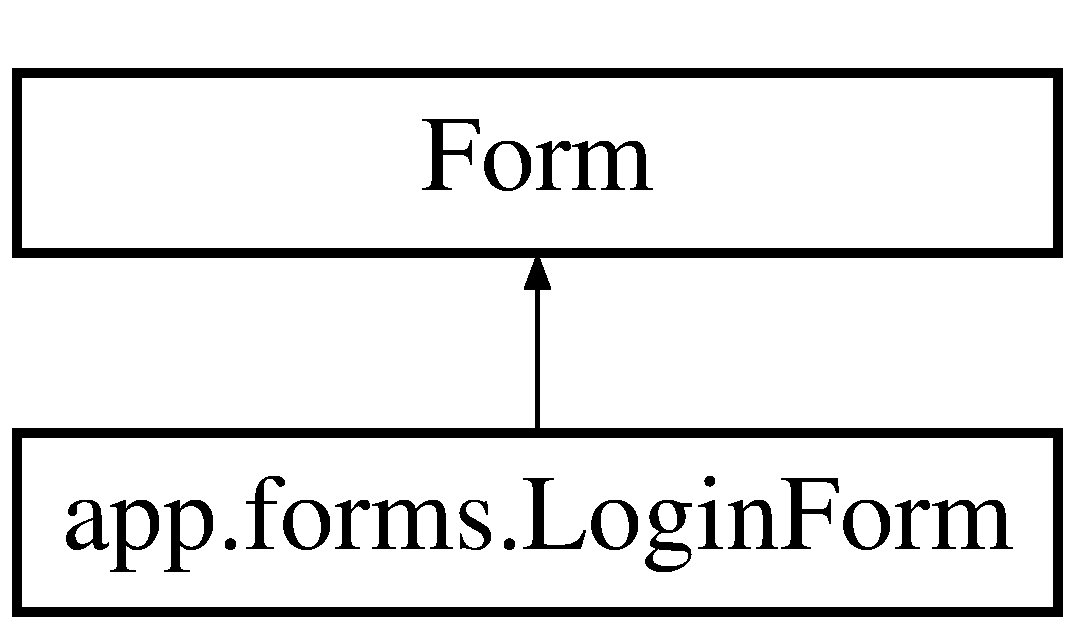
\includegraphics[height=2.000000cm]{classapp_1_1forms_1_1LoginForm}
\end{center}
\end{figure}


\subsection{Detailed Description}
Form which requires user credentials to submit. 

\hyperlink{classapp_1_1forms_1_1LoginForm}{Login\+Form} enforces the presence of both a username and a password. The parent class Form defines the interface to flask. The variables below define fields in the form, and how they are validated. 

The documentation for this class was generated from the following file\+:\begin{DoxyCompactItemize}
\item 
\hyperlink{forms_8py}{forms.\+py}\end{DoxyCompactItemize}

\hypertarget{classapp_1_1Month_1_1Month}{}\section{app.\+Month.\+Month Class Reference}
\label{classapp_1_1Month_1_1Month}\index{app.\+Month.\+Month@{app.\+Month.\+Month}}


A month which possesses a list of days, and calculates lists of weeks.  


\subsection*{Public Member Functions}
\begin{DoxyCompactItemize}
\item 
def \hyperlink{classapp_1_1Month_1_1Month_a37375e0ac2693a9b4701dacd7de23a5a}{\+\_\+\+\_\+init\+\_\+\+\_\+} (self, name, days, year)
\begin{DoxyCompactList}\small\item\em Initializes a month object. \end{DoxyCompactList}\item 
def \hyperlink{classapp_1_1Month_1_1Month_a0577a1a22deaa2fba3b7e3f4a7aecabb}{set\+Prev} (self, month)
\begin{DoxyCompactList}\small\item\em sets the previous month, updates the first week \end{DoxyCompactList}\item 
def \hyperlink{classapp_1_1Month_1_1Month_aa2f066e84d3a0118b9279ac18adc53d0}{set\+Next} (self, month)
\begin{DoxyCompactList}\small\item\em sets the next month, updates the last week \end{DoxyCompactList}\item 
def \hyperlink{classapp_1_1Month_1_1Month_aa4cb140eba9322590e2e20e6366b6ef7}{get\+Day} (self, date)
\begin{DoxyCompactList}\small\item\em Gets the day at a certain date. \end{DoxyCompactList}\end{DoxyCompactItemize}
\subsection*{Public Attributes}
\begin{DoxyCompactItemize}
\item 
{\bfseries name}\hypertarget{classapp_1_1Month_1_1Month_ad8bb2df501f5c1371b5315c2f6e3035f}{}\label{classapp_1_1Month_1_1Month_ad8bb2df501f5c1371b5315c2f6e3035f}

\item 
{\bfseries days}\hypertarget{classapp_1_1Month_1_1Month_ae9e6419b902f69c5a08866a2d598dfca}{}\label{classapp_1_1Month_1_1Month_ae9e6419b902f69c5a08866a2d598dfca}

\item 
{\bfseries num\+Days}\hypertarget{classapp_1_1Month_1_1Month_ae05ee940bd515dbf90455ab77221a785}{}\label{classapp_1_1Month_1_1Month_ae05ee940bd515dbf90455ab77221a785}

\item 
{\bfseries year}\hypertarget{classapp_1_1Month_1_1Month_a6b1efc7cf987876f70dda6540dd5ff7b}{}\label{classapp_1_1Month_1_1Month_a6b1efc7cf987876f70dda6540dd5ff7b}

\item 
{\bfseries weeks}\hypertarget{classapp_1_1Month_1_1Month_aa7666a88a2282ba3172d2fdc3f26c301}{}\label{classapp_1_1Month_1_1Month_aa7666a88a2282ba3172d2fdc3f26c301}

\item 
{\bfseries prev}\hypertarget{classapp_1_1Month_1_1Month_a53b0c7e0822baa2ec552d7fbd52625c1}{}\label{classapp_1_1Month_1_1Month_a53b0c7e0822baa2ec552d7fbd52625c1}

\item 
{\bfseries next}\hypertarget{classapp_1_1Month_1_1Month_ada35442c38ecaadf5a299f6295ead36e}{}\label{classapp_1_1Month_1_1Month_ada35442c38ecaadf5a299f6295ead36e}

\end{DoxyCompactItemize}


\subsection{Detailed Description}
A month which possesses a list of days, and calculates lists of weeks. 

\begin{DoxyAuthor}{Author}
Grant Jurgensen
\end{DoxyAuthor}
A container for a month, holds the associated days, as well as weeks within it. In order for the weeks to all be full (7 days, sunday-\/saturday), the month must be made aware of its previous and next months. 

\subsection{Constructor \& Destructor Documentation}
\index{app\+::\+Month\+::\+Month@{app\+::\+Month\+::\+Month}!\+\_\+\+\_\+init\+\_\+\+\_\+@{\+\_\+\+\_\+init\+\_\+\+\_\+}}
\index{\+\_\+\+\_\+init\+\_\+\+\_\+@{\+\_\+\+\_\+init\+\_\+\+\_\+}!app\+::\+Month\+::\+Month@{app\+::\+Month\+::\+Month}}
\subsubsection[{\texorpdfstring{\+\_\+\+\_\+init\+\_\+\+\_\+(self, name, days, year)}{\_\_init\_\_(self, name, days, year)}}]{\setlength{\rightskip}{0pt plus 5cm}app.\+Month.\+Month.\+\_\+\+\_\+init\+\_\+\+\_\+ (
\begin{DoxyParamCaption}
\item[{}]{self, }
\item[{}]{name, }
\item[{}]{days, }
\item[{}]{year}
\end{DoxyParamCaption}
)}\hypertarget{classapp_1_1Month_1_1Month_a37375e0ac2693a9b4701dacd7de23a5a}{}\label{classapp_1_1Month_1_1Month_a37375e0ac2693a9b4701dacd7de23a5a}


Initializes a month object. 


\begin{DoxyParams}[1]{Parameters}
\mbox{\tt in}  & {\em name} & A string value of the month\textquotesingle{}s name, e.\+g \textquotesingle{}January\textquotesingle{} \\
\hline
\mbox{\tt in}  & {\em days} & A list of days which the month contains \\
\hline
\mbox{\tt in}  & {\em year} & The year object that the month belongs to \\
\hline
\mbox{\tt out}  & {\em return} & The initialized month object\\
\hline
\end{DoxyParams}
Initializes a \hyperlink{classapp_1_1Month_1_1Month}{Month} object. Stores its name, year, and days. Creates a first draft of its weeks (The weeks won\textquotesingle{}t neccessary be full until the month is made aware of its previous and next month). 

\subsection{Member Function Documentation}
\index{app\+::\+Month\+::\+Month@{app\+::\+Month\+::\+Month}!get\+Day@{get\+Day}}
\index{get\+Day@{get\+Day}!app\+::\+Month\+::\+Month@{app\+::\+Month\+::\+Month}}
\subsubsection[{\texorpdfstring{get\+Day(self, date)}{getDay(self, date)}}]{\setlength{\rightskip}{0pt plus 5cm}app.\+Month.\+Month.\+get\+Day (
\begin{DoxyParamCaption}
\item[{}]{self, }
\item[{}]{date}
\end{DoxyParamCaption}
)}\hypertarget{classapp_1_1Month_1_1Month_aa4cb140eba9322590e2e20e6366b6ef7}{}\label{classapp_1_1Month_1_1Month_aa4cb140eba9322590e2e20e6366b6ef7}


Gets the day at a certain date. 


\begin{DoxyParams}[1]{Parameters}
\mbox{\tt in}  & {\em date} & An integer value, the date of the day, e.\+g 5 for the 5th \\
\hline
\mbox{\tt out}  & {\em return} & Returns the day if the date was within the bounds of the month otherwise it returns None \\
\hline
\end{DoxyParams}
\index{app\+::\+Month\+::\+Month@{app\+::\+Month\+::\+Month}!set\+Next@{set\+Next}}
\index{set\+Next@{set\+Next}!app\+::\+Month\+::\+Month@{app\+::\+Month\+::\+Month}}
\subsubsection[{\texorpdfstring{set\+Next(self, month)}{setNext(self, month)}}]{\setlength{\rightskip}{0pt plus 5cm}app.\+Month.\+Month.\+set\+Next (
\begin{DoxyParamCaption}
\item[{}]{self, }
\item[{}]{month}
\end{DoxyParamCaption}
)}\hypertarget{classapp_1_1Month_1_1Month_aa2f066e84d3a0118b9279ac18adc53d0}{}\label{classapp_1_1Month_1_1Month_aa2f066e84d3a0118b9279ac18adc53d0}


sets the next month, updates the last week 


\begin{DoxyParams}[1]{Parameters}
\mbox{\tt in}  & {\em month} & The month object which imidiately follows this month \\
\hline
\mbox{\tt out}  & {\em return} & Returns true if it was able to complete the last week, false otherwise\\
\hline
\end{DoxyParams}
Sets the next month, and then if the last week of the month isn\textquotesingle{}t already full, it will work forward and continuously add to the back of the last week until it reaches \char`\"{}\+Saturday\char`\"{}. Returns true if successful, false otherwise \index{app\+::\+Month\+::\+Month@{app\+::\+Month\+::\+Month}!set\+Prev@{set\+Prev}}
\index{set\+Prev@{set\+Prev}!app\+::\+Month\+::\+Month@{app\+::\+Month\+::\+Month}}
\subsubsection[{\texorpdfstring{set\+Prev(self, month)}{setPrev(self, month)}}]{\setlength{\rightskip}{0pt plus 5cm}app.\+Month.\+Month.\+set\+Prev (
\begin{DoxyParamCaption}
\item[{}]{self, }
\item[{}]{month}
\end{DoxyParamCaption}
)}\hypertarget{classapp_1_1Month_1_1Month_a0577a1a22deaa2fba3b7e3f4a7aecabb}{}\label{classapp_1_1Month_1_1Month_a0577a1a22deaa2fba3b7e3f4a7aecabb}


sets the previous month, updates the first week 


\begin{DoxyParams}[1]{Parameters}
\mbox{\tt in}  & {\em month} & The month object which proceeds this month \\
\hline
\mbox{\tt out}  & {\em return} & Returns true if it was able to complete the first week, false otherwise\\
\hline
\end{DoxyParams}
Sets the previous month, and then if the first week of the month isn\textquotesingle{}t already full, it will work backwards and continuously add to the front of the first week until it reaches \char`\"{}\+Sunday\char`\"{}. Returns true if successful, false otherwise 

The documentation for this class was generated from the following file\+:\begin{DoxyCompactItemize}
\item 
\hyperlink{Month_8py}{Month.\+py}\end{DoxyCompactItemize}

\hypertarget{classapp_1_1Year_1_1Year}{}\section{app.\+Year.\+Year Class Reference}
\label{classapp_1_1Year_1_1Year}\index{app.\+Year.\+Year@{app.\+Year.\+Year}}


Generates a year, including the months, weeks, and days contained with in it.  


\subsection*{Public Member Functions}
\begin{DoxyCompactItemize}
\item 
def \hyperlink{classapp_1_1Year_1_1Year_a7137b85e17cf71cb61a4eaf1b46be837}{\+\_\+\+\_\+init\+\_\+\+\_\+} (self, name)
\begin{DoxyCompactList}\small\item\em Initializes a \hyperlink{classapp_1_1Year_1_1Year}{Year} object. \end{DoxyCompactList}\item 
def \hyperlink{classapp_1_1Year_1_1Year_a4fc579bd5b473c0898ae41902b084f80}{set\+Prev} (self, year)
\begin{DoxyCompactList}\small\item\em makes the year object aware of its previous year \end{DoxyCompactList}\item 
def \hyperlink{classapp_1_1Year_1_1Year_aa68562faa318617f6c4c90919d27d195}{set\+Next} (self, year)
\begin{DoxyCompactList}\small\item\em makes the year object aware of the next year \end{DoxyCompactList}\item 
def \hyperlink{classapp_1_1Year_1_1Year_ad1d40047ed4bff44be11156937427ceb}{get\+Month} (self, month\+Name)
\begin{DoxyCompactList}\small\item\em gets the month object via the name of the month \end{DoxyCompactList}\end{DoxyCompactItemize}
\subsection*{Public Attributes}
\begin{DoxyCompactItemize}
\item 
{\bfseries name}\hypertarget{classapp_1_1Year_1_1Year_acea84e2a70bc0ee6dcf861844d07d0ce}{}\label{classapp_1_1Year_1_1Year_acea84e2a70bc0ee6dcf861844d07d0ce}

\item 
{\bfseries months}\hypertarget{classapp_1_1Year_1_1Year_a9fb96c5085ea992d63f8b101874d2598}{}\label{classapp_1_1Year_1_1Year_a9fb96c5085ea992d63f8b101874d2598}

\item 
{\bfseries prev}\hypertarget{classapp_1_1Year_1_1Year_a605ebe3be0030f87084b98e2b76bd5b6}{}\label{classapp_1_1Year_1_1Year_a605ebe3be0030f87084b98e2b76bd5b6}

\item 
{\bfseries next}\hypertarget{classapp_1_1Year_1_1Year_ab3c168ef1e6412e3dbb719cf7928e6b3}{}\label{classapp_1_1Year_1_1Year_ab3c168ef1e6412e3dbb719cf7928e6b3}

\end{DoxyCompactItemize}


\subsection{Detailed Description}
Generates a year, including the months, weeks, and days contained with in it. 

\begin{DoxyAuthor}{Author}
Grant Jurgensen
\end{DoxyAuthor}
Generates a full year (January 1st through December 31), and auto-\/fills itself with the months and days within it. It can \char`\"{}link\char`\"{} with other years, so that the weeks within its months are able to bleed over between the year boundaries. 

\subsection{Constructor \& Destructor Documentation}
\index{app\+::\+Year\+::\+Year@{app\+::\+Year\+::\+Year}!\+\_\+\+\_\+init\+\_\+\+\_\+@{\+\_\+\+\_\+init\+\_\+\+\_\+}}
\index{\+\_\+\+\_\+init\+\_\+\+\_\+@{\+\_\+\+\_\+init\+\_\+\+\_\+}!app\+::\+Year\+::\+Year@{app\+::\+Year\+::\+Year}}
\subsubsection[{\texorpdfstring{\+\_\+\+\_\+init\+\_\+\+\_\+(self, name)}{\_\_init\_\_(self, name)}}]{\setlength{\rightskip}{0pt plus 5cm}app.\+Year.\+Year.\+\_\+\+\_\+init\+\_\+\+\_\+ (
\begin{DoxyParamCaption}
\item[{}]{self, }
\item[{}]{name}
\end{DoxyParamCaption}
)}\hypertarget{classapp_1_1Year_1_1Year_a7137b85e17cf71cb61a4eaf1b46be837}{}\label{classapp_1_1Year_1_1Year_a7137b85e17cf71cb61a4eaf1b46be837}


Initializes a \hyperlink{classapp_1_1Year_1_1Year}{Year} object. 


\begin{DoxyParams}[1]{Parameters}
\mbox{\tt in}  & {\em name} & An integer value corresponding to the year, e.\+g. 2016 \\
\hline
\mbox{\tt out}  & {\em return} & The initialized \hyperlink{classapp_1_1Year_1_1Year}{Year} object\\
\hline
\end{DoxyParams}
Initializes a \hyperlink{classapp_1_1Year_1_1Year}{Year} object. Calculates whether it is a leap year, and adjusts the months lengths if so. Calculates the weekday of the first day of the year in order to have a reference point for all future days created. Iterates through 12 months, creates each month and fills it with the appropriate days. 

\subsection{Member Function Documentation}
\index{app\+::\+Year\+::\+Year@{app\+::\+Year\+::\+Year}!get\+Month@{get\+Month}}
\index{get\+Month@{get\+Month}!app\+::\+Year\+::\+Year@{app\+::\+Year\+::\+Year}}
\subsubsection[{\texorpdfstring{get\+Month(self, month\+Name)}{getMonth(self, monthName)}}]{\setlength{\rightskip}{0pt plus 5cm}app.\+Year.\+Year.\+get\+Month (
\begin{DoxyParamCaption}
\item[{}]{self, }
\item[{}]{month\+Name}
\end{DoxyParamCaption}
)}\hypertarget{classapp_1_1Year_1_1Year_ad1d40047ed4bff44be11156937427ceb}{}\label{classapp_1_1Year_1_1Year_ad1d40047ed4bff44be11156937427ceb}


gets the month object via the name of the month 


\begin{DoxyParams}[1]{Parameters}
\mbox{\tt in}  & {\em month\+Name} & A string value for name of the month \\
\hline
\mbox{\tt out}  & {\em return} & Returns the month object of that name, or if none is found, None\\
\hline
\end{DoxyParams}
Searches all of its months looking for a match to the month\+Name argument. If it finds one, it will return that month. Otherwise, it will return None. \index{app\+::\+Year\+::\+Year@{app\+::\+Year\+::\+Year}!set\+Next@{set\+Next}}
\index{set\+Next@{set\+Next}!app\+::\+Year\+::\+Year@{app\+::\+Year\+::\+Year}}
\subsubsection[{\texorpdfstring{set\+Next(self, year)}{setNext(self, year)}}]{\setlength{\rightskip}{0pt plus 5cm}app.\+Year.\+Year.\+set\+Next (
\begin{DoxyParamCaption}
\item[{}]{self, }
\item[{}]{year}
\end{DoxyParamCaption}
)}\hypertarget{classapp_1_1Year_1_1Year_aa68562faa318617f6c4c90919d27d195}{}\label{classapp_1_1Year_1_1Year_aa68562faa318617f6c4c90919d27d195}


makes the year object aware of the next year 


\begin{DoxyParams}[1]{Parameters}
\mbox{\tt in}  & {\em year} & A year object which imidiately follows this year object\\
\hline
\end{DoxyParams}
In order for the weeks within the months to be full weeks (sunday-\/saturday), the year object must be aware of its next year. This way the weeks may bleed over into the next year if neccessary \index{app\+::\+Year\+::\+Year@{app\+::\+Year\+::\+Year}!set\+Prev@{set\+Prev}}
\index{set\+Prev@{set\+Prev}!app\+::\+Year\+::\+Year@{app\+::\+Year\+::\+Year}}
\subsubsection[{\texorpdfstring{set\+Prev(self, year)}{setPrev(self, year)}}]{\setlength{\rightskip}{0pt plus 5cm}app.\+Year.\+Year.\+set\+Prev (
\begin{DoxyParamCaption}
\item[{}]{self, }
\item[{}]{year}
\end{DoxyParamCaption}
)}\hypertarget{classapp_1_1Year_1_1Year_a4fc579bd5b473c0898ae41902b084f80}{}\label{classapp_1_1Year_1_1Year_a4fc579bd5b473c0898ae41902b084f80}


makes the year object aware of its previous year 


\begin{DoxyParams}[1]{Parameters}
\mbox{\tt in}  & {\em year} & A year object which that precedes this year object\\
\hline
\end{DoxyParams}
In order for the weeks within the months to be full weeks (sunday-\/saturday), the year object must be aware of its previous year. This way the weeks may bleed over into the previous year if neccessary 

The documentation for this class was generated from the following file\+:\begin{DoxyCompactItemize}
\item 
\hyperlink{Year_8py}{Year.\+py}\end{DoxyCompactItemize}

\chapter{File Documentation}
\hypertarget{____init_____8py}{}\section{\+\_\+\+\_\+init\+\_\+\+\_\+.\+py File Reference}
\label{____init_____8py}\index{\+\_\+\+\_\+init\+\_\+\+\_\+.\+py@{\+\_\+\+\_\+init\+\_\+\+\_\+.\+py}}


Decouples app instantiation and configuration from use.  


\subsection*{Variables}
\begin{DoxyCompactItemize}
\item 
{\bfseries app.\+app} = Flask(\+\_\+\+\_\+name\+\_\+\+\_\+)\hypertarget{____init_____8py_a675b4ea702c13dc4b8c05f985a25b496}{}\label{____init_____8py_a675b4ea702c13dc4b8c05f985a25b496}

\item 
{\bfseries app.\+secret\+\_\+key}\hypertarget{____init_____8py_adca7658ff5c9024a5353574d2c01cbd2}{}\label{____init_____8py_adca7658ff5c9024a5353574d2c01cbd2}

\end{DoxyCompactItemize}


\subsection{Detailed Description}
Decouples app instantiation and configuration from use. 

\begin{DoxyAuthor}{Author}
Stephen Longofono
\end{DoxyAuthor}
This module exists to decouple the Flask app object and its configuration from the views and other pieces of the project. It should not be run directly; it will be called by \textquotesingle{}run.\+py\textquotesingle{} when it has finished running its setup steps. 
\hypertarget{Calendar_8py}{}\section{Calendar.\+py File Reference}
\label{Calendar_8py}\index{Calendar.\+py@{Calendar.\+py}}


Holds two years, and keeps track of the currently selected day.  


\subsection*{Classes}
\begin{DoxyCompactItemize}
\item 
class \hyperlink{classapp_1_1Calendar_1_1Calendar}{app.\+Calendar.\+Calendar}
\begin{DoxyCompactList}\small\item\em Holds two years, and keeps track of the currently selected day. \end{DoxyCompactList}\end{DoxyCompactItemize}


\subsection{Detailed Description}
Holds two years, and keeps track of the currently selected day. 

\begin{DoxyAuthor}{Author}
Grant Jurgensen 
\end{DoxyAuthor}

\hypertarget{Day_8py}{}\section{Day.\+py File Reference}
\label{Day_8py}\index{Day.\+py@{Day.\+py}}


A day with a list of details.  


\subsection*{Classes}
\begin{DoxyCompactItemize}
\item 
class \hyperlink{classapp_1_1Day_1_1Day}{app.\+Day.\+Day}
\begin{DoxyCompactList}\small\item\em A day with a list of details. \end{DoxyCompactList}\end{DoxyCompactItemize}


\subsection{Detailed Description}
A day with a list of details. 

\begin{DoxyAuthor}{Author}
Grant Jurgensen 
\end{DoxyAuthor}

\hypertarget{forms_8py}{}\section{forms.\+py File Reference}
\label{forms_8py}\index{forms.\+py@{forms.\+py}}


Defines custom forms for server-\/side validation.  


\subsection*{Classes}
\begin{DoxyCompactItemize}
\item 
class \hyperlink{classapp_1_1forms_1_1LoginForm}{app.\+forms.\+Login\+Form}
\begin{DoxyCompactList}\small\item\em Form which requires user credentials to submit. \end{DoxyCompactList}\end{DoxyCompactItemize}
\subsection*{Variables}
\begin{DoxyCompactItemize}
\item 
{\bfseries app.\+forms.\+uname} = String\+Field(\textquotesingle{}uname\textquotesingle{}, validators=\mbox{[}Required()\mbox{]})\hypertarget{forms_8py_a392d934daf562344a902a800b6effb12}{}\label{forms_8py_a392d934daf562344a902a800b6effb12}

\item 
{\bfseries app.\+forms.\+pword} = Password\+Field(\textquotesingle{}pword\textquotesingle{}, validators=\mbox{[}Required()\mbox{]})\hypertarget{forms_8py_a90ae12ebd3969daaf7ea766e5e6ffda6}{}\label{forms_8py_a90ae12ebd3969daaf7ea766e5e6ffda6}

\end{DoxyCompactItemize}


\subsection{Detailed Description}
Defines custom forms for server-\/side validation. 

\begin{DoxyAuthor}{Author}
Stephen Longofono
\end{DoxyAuthor}
This module defines a custom form used for accepting and filtering input on the server side portion of our project. Specifically, we use it to gather login information. 
\hypertarget{Month_8py}{}\section{Month.\+py File Reference}
\label{Month_8py}\index{Month.\+py@{Month.\+py}}


A month which possesses a list of days, and calculates lists of weeks.  


\subsection*{Classes}
\begin{DoxyCompactItemize}
\item 
class \hyperlink{classapp_1_1Month_1_1Month}{app.\+Month.\+Month}
\begin{DoxyCompactList}\small\item\em A month which possesses a list of days, and calculates lists of weeks. \end{DoxyCompactList}\end{DoxyCompactItemize}


\subsection{Detailed Description}
A month which possesses a list of days, and calculates lists of weeks. 

\begin{DoxyAuthor}{Author}
Grant Jurgensen 
\end{DoxyAuthor}

\hypertarget{views_8py}{}\section{views.\+py File Reference}
\label{views_8py}\index{views.\+py@{views.\+py}}


Manages login, session, and server-\/side interaction of project pages.  


\subsection*{Functions}
\begin{DoxyCompactItemize}
\item 
def {\bfseries app.\+views.\+delete} ()\hypertarget{views_8py_a33f9468136d69c9ef1dd37b3f469b690}{}\label{views_8py_a33f9468136d69c9ef1dd37b3f469b690}

\item 
def {\bfseries app.\+views.\+index} (view=None)\hypertarget{views_8py_acaf59a2cf0ccf654ea7d427ce34bd646}{}\label{views_8py_acaf59a2cf0ccf654ea7d427ce34bd646}

\item 
def \hyperlink{views_8py_ad7a2f71759324c512f85a8c3b3247643}{app.\+views.\+login} ()
\begin{DoxyCompactList}\small\item\em login request behavior \end{DoxyCompactList}\item 
def \hyperlink{views_8py_aab028cc1ea5e110fd0123581e9119b01}{app.\+views.\+logout} ()
\begin{DoxyCompactList}\small\item\em logout request behavior \end{DoxyCompactList}\item 
def \hyperlink{views_8py_a183993ab7922bdd22fa9f8aa657a9c4f}{app.\+views.\+process} ()
\begin{DoxyCompactList}\small\item\em processes changes to details in calendar and logfile \end{DoxyCompactList}\item 
def \hyperlink{views_8py_accb2808eb43d7b94fb79c6d0ab01c5c3}{app.\+views.\+view\+Change} ()
\begin{DoxyCompactList}\small\item\em handles routing for changing the client\textquotesingle{}s view of the current day/week/month/year \end{DoxyCompactList}\item 
def {\bfseries app.\+views.\+change\+Focus\+Day} ()\hypertarget{views_8py_a88b84f0e4c7bedd243c8a684e8db0c1e}{}\label{views_8py_a88b84f0e4c7bedd243c8a684e8db0c1e}

\item 
def {\bfseries app.\+views.\+change\+Focus\+Month} ()\hypertarget{views_8py_a36b428f7e7c0d1d77645eefee56365a2}{}\label{views_8py_a36b428f7e7c0d1d77645eefee56365a2}

\item 
def {\bfseries app.\+views.\+page\+\_\+not\+\_\+found} (e)\hypertarget{views_8py_abe711a5ac5302330fadb2bc6870e0c52}{}\label{views_8py_abe711a5ac5302330fadb2bc6870e0c52}

\end{DoxyCompactItemize}
\subsection*{Variables}
\begin{DoxyCompactItemize}
\item 
{\bfseries app.\+views.\+calendar\+\_\+obj} = Calendar.\+Calendar(2016, 2017, \textquotesingle{}logfile.\+txt\textquotesingle{})\hypertarget{views_8py_ab2bcd64276d31af0674c8ac2f9503ecf}{}\label{views_8py_ab2bcd64276d31af0674c8ac2f9503ecf}

\item 
{\bfseries app.\+views.\+methods}\hypertarget{views_8py_a0d1cbd1cb152e18473257553e90a9097}{}\label{views_8py_a0d1cbd1cb152e18473257553e90a9097}

\end{DoxyCompactItemize}


\subsection{Detailed Description}
Manages login, session, and server-\/side interaction of project pages. 

\begin{DoxyAuthor}{Author}
Stephen Longofono
\end{DoxyAuthor}
\begin{DoxyVerb}This file defines all the viable addresses for our project webpages and how
\end{DoxyVerb}
 they will interact on the server side. After directing visitors through a login process, a session is established to designate that a user is authenticated.

A calendar object is maintained for the lifetime of the server, created from scratch and populated with details from a logfile if present. There is only one user, so for this iteration there is only one logfile.

Each method is marked with a decorator, indicating that Flask should call that method when the address argument of app.\+route() is accessed by the user. Most methods handle the control of what the user can and cannot see or otherwise access. The process method interacts with client-\/side Javascript to parse and interpret input. Javascript is able to access objects passed into the render\+\_\+template() method, and responds to the server via J\+S\+ON. 

\subsection{Function Documentation}
\index{views.\+py@{views.\+py}!login@{login}}
\index{login@{login}!views.\+py@{views.\+py}}
\subsubsection[{\texorpdfstring{login()}{login()}}]{\setlength{\rightskip}{0pt plus 5cm}app.\+views.\+login (
\begin{DoxyParamCaption}
{}
\end{DoxyParamCaption}
)}\hypertarget{views_8py_file_ad7a2f71759324c512f85a8c3b3247643}{}\label{views_8py_file_ad7a2f71759324c512f85a8c3b3247643}


login request behavior 


\begin{DoxyParams}[1]{Parameters}
\mbox{\tt in}  & {\em session} & An implicit variable generated by flask, acts as a cryptographically signed cookie to store any information which should be preserved across requests \\
\hline
\mbox{\tt out}  & {\em return} & Redirects to the index() method, or A rendered H\+T\+ML document of the login page if the login credentials are invalid\\
\hline
\end{DoxyParams}
The login will validate the user\textquotesingle{}s input using a Login\+Form and create a session for the user if the credentials are valid. The user and session are then redirected to the index() method. If the user credentials are invalid, the login page is re-\/rendered and feedback is provided. \index{views.\+py@{views.\+py}!logout@{logout}}
\index{logout@{logout}!views.\+py@{views.\+py}}
\subsubsection[{\texorpdfstring{logout()}{logout()}}]{\setlength{\rightskip}{0pt plus 5cm}app.\+views.\+logout (
\begin{DoxyParamCaption}
{}
\end{DoxyParamCaption}
)}\hypertarget{views_8py_file_aab028cc1ea5e110fd0123581e9119b01}{}\label{views_8py_file_aab028cc1ea5e110fd0123581e9119b01}


logout request behavior 


\begin{DoxyParams}[1]{Parameters}
\mbox{\tt in}  & {\em session} & An implicit variable generated by flask, acts as a cryptographically signed cookie to store any information which should be preserved across requests \\
\hline
\mbox{\tt out}  & {\em return} & Redirects to the \hyperlink{views_8py_ad7a2f71759324c512f85a8c3b3247643}{login()} method\\
\hline
\end{DoxyParams}
The logout will clear all data from the session field, and redirect to the \hyperlink{views_8py_ad7a2f71759324c512f85a8c3b3247643}{login()} method \index{views.\+py@{views.\+py}!process@{process}}
\index{process@{process}!views.\+py@{views.\+py}}
\subsubsection[{\texorpdfstring{process()}{process()}}]{\setlength{\rightskip}{0pt plus 5cm}app.\+views.\+process (
\begin{DoxyParamCaption}
{}
\end{DoxyParamCaption}
)}\hypertarget{views_8py_file_a183993ab7922bdd22fa9f8aa657a9c4f}{}\label{views_8py_file_a183993ab7922bdd22fa9f8aa657a9c4f}


processes changes to details in calendar and logfile 


\begin{DoxyParams}[1]{Parameters}
\mbox{\tt in}  & {\em J\+S\+ON} & This is an implicit parameter passed along via Flask\textquotesingle{}s request construct. It is reconstructed as a dictionary on entry to this method. \\
\hline
\mbox{\tt out}  & {\em return} & Returns a J\+S\+O\+N-\/style object representing the status\\
\hline
\end{DoxyParams}
The process method will attempt to parse J\+S\+O\+N-\/style form data sent from the client-\/side representing a day and its current details. The day in questions is located using the month and year passed in, and its details are replaced by those parsed from the J\+S\+ON.

Assumes \textquotesingle{}day\textquotesingle{}, \textquotesingle{}month\textquotesingle{}, \textquotesingle{}year\textquotesingle{}, and \textquotesingle{}date\textquotesingle{} are present \index{views.\+py@{views.\+py}!view\+Change@{view\+Change}}
\index{view\+Change@{view\+Change}!views.\+py@{views.\+py}}
\subsubsection[{\texorpdfstring{view\+Change()}{viewChange()}}]{\setlength{\rightskip}{0pt plus 5cm}app.\+views.\+view\+Change (
\begin{DoxyParamCaption}
{}
\end{DoxyParamCaption}
)}\hypertarget{views_8py_file_accb2808eb43d7b94fb79c6d0ab01c5c3}{}\label{views_8py_file_accb2808eb43d7b94fb79c6d0ab01c5c3}


handles routing for changing the client\textquotesingle{}s view of the current day/week/month/year 


\begin{DoxyParams}[1]{Parameters}
\mbox{\tt in}  & {\em J\+S\+ON} & This is an implicit parameter passed along via Flask\textquotesingle{}s request construct. It is reconstructed as a dictionary on entry to this method. \\
\hline
\mbox{\tt out}  & {\em return} & Returns a J\+S\+O\+N-\/style object representing the status and a link to redirect to for client-\/side\\
\hline
\end{DoxyParams}
The view\+Change method will attempt to parse J\+S\+O\+N-\/style form data sent from the client-\/side representing a new view request. Acceptable values for the \textquotesingle{}view\textquotesingle{} key are \textquotesingle{}next\textquotesingle{}, \textquotesingle{}prev\textquotesingle{}, \textquotesingle{}day\textquotesingle{}, \textquotesingle{}week\textquotesingle{}, \textquotesingle{}month\textquotesingle{}, or \textquotesingle{}year\textquotesingle{}.

When necessary, the server-\/side calendar object is updated to point to the next or previous day. In this case, a link for the index in day view is provided in the return. Otherwise, a link to index is provided with a view matching the view specfified by the J\+S\+ON.

Assumes \textquotesingle{}view\textquotesingle{} is present and has a value. 
\hypertarget{Year_8py}{}\section{Year.\+py File Reference}
\label{Year_8py}\index{Year.\+py@{Year.\+py}}


Generates a year, including the months, weeks, and days contained with in it.  


\subsection*{Classes}
\begin{DoxyCompactItemize}
\item 
class \hyperlink{classapp_1_1Year_1_1Year}{app.\+Year.\+Year}
\begin{DoxyCompactList}\small\item\em Generates a year, including the months, weeks, and days contained with in it. \end{DoxyCompactList}\end{DoxyCompactItemize}


\subsection{Detailed Description}
Generates a year, including the months, weeks, and days contained with in it. 

\begin{DoxyAuthor}{Author}
Grant Jurgensen 
\end{DoxyAuthor}

%--- End generated contents ---

% Index
\backmatter
\newpage
\phantomsection
\clearemptydoublepage
\addcontentsline{toc}{chapter}{Index}
\printindex

\end{document}
